\subsection{Fuel salt reprocessing system}

\begin{frame}
  \frametitle{Fuel salt reprocessing system overview: gas separation}
  Gaseous fission products (e.g., Xe, Kr) must be removed from the fuel salt 
  to avoid reactor
poisoning. 
  
      \begin{columns}
      	\column[t]{4.5cm}
    \begin{block}{Noble gases removal process:}
      \begin{enumerate}
      	\item bubble generator injects He bubbles in the salt stream
      	\item noble gases migrate to the He bubbles due to their insolubility 
      	in salt
      	\item gas separator discharges the poison-rich bubbles from the salt
      \end{enumerate}
    \end{block}    	
      	
     	\column[t]{7cm}
  \begin{figure}[t]
	  \centering
	  		\vspace{-8mm}
		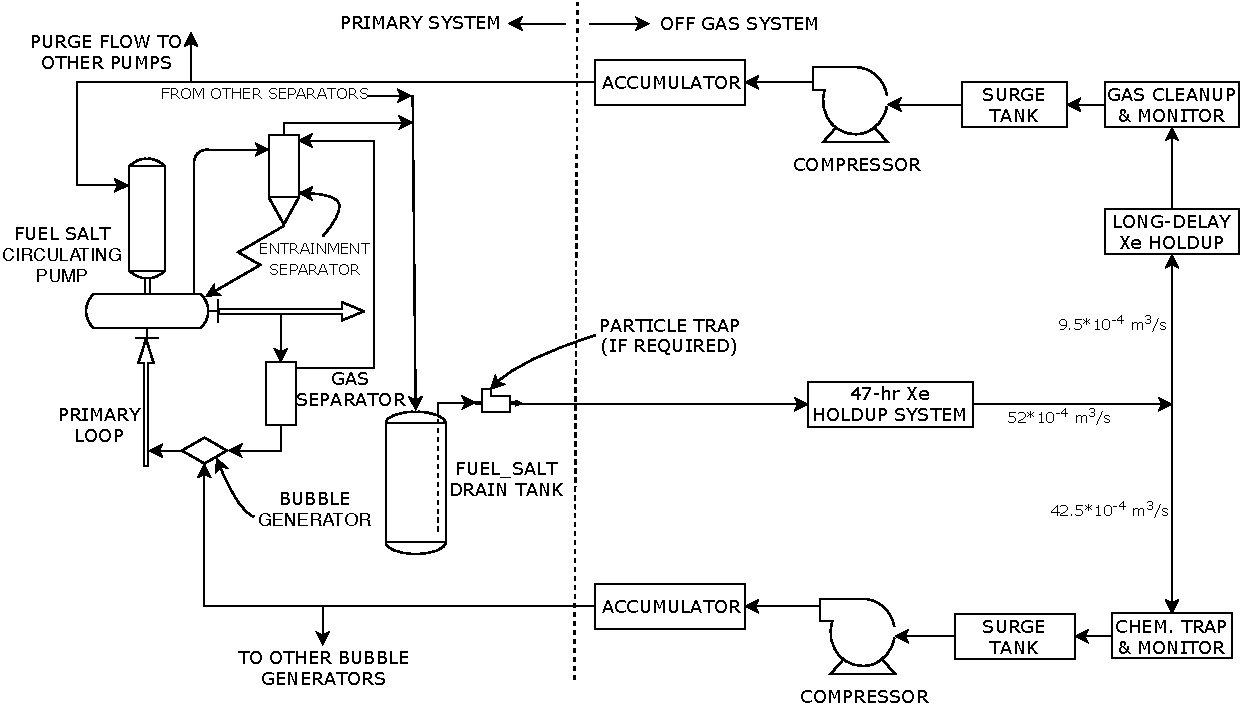
\includegraphics[width=1.03\textwidth]{../figures/gas_separation.pdf}
	\caption{Schematic flow diagram of the \gls{MSBR} gas separation system 
	(figure reproduced from Robertson \emph{et al.}  
	\cite{robertson_conceptual_1971}).} 
    \end{figure}

	\end{columns}
\end{frame}

\begin{frame}
  \frametitle{Mathematical model for gas separation efficiency}
  		\vspace{-1mm}
Xenon removal efficiency ($\epsilon_{Xe}$) in a gas separation system is 
\cite{peebles_removal_1968}:
\begin{align}
& \qquad\qquad \epsilon_{Xe} = \frac{1-e^{-\beta}}{1+\alpha} \nonumber \\
\alpha &= \frac{RTQ_{L}}{HQ_{G}} \nonumber \\
\beta &= \frac{K_L a A_C L (1+\alpha)}{Q_{L}} \nonumber \\
Q_{L}&= \mbox{volumetric salt flow rate} \nonumber \\
Q_{G}&= \mbox{volumetric helium flow rate} \nonumber \\
H &= \mbox{Henry's law constant} \nonumber \\
a &= \mbox{gas-liquid interfacial area} \nonumber \\
K_L &= \mbox{liquid phase mass transfer coefficient.} \nonumber
\end{align}
		\vspace{-5mm}
  \begin{figure}[t]
	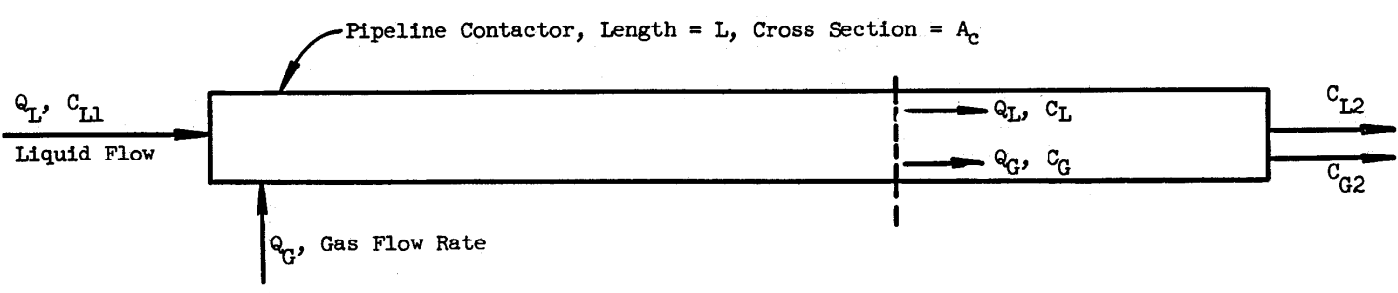
\includegraphics[width=0.66\textwidth]{./images/pipeline_contactor.png}
	\vspace{-2mm}
	\caption{Flow diagram for gas separator (figure reproduced from Peebles 
		\emph{et al.} \cite{peebles_removal_1968}).}
\end{figure}

\end{frame}


\begin{frame}
\frametitle{Fuel processing system overview: rare earths and Pa removal}
	\begin{figure}[htp!] % replace 't' with 'b' to 
		\centering
			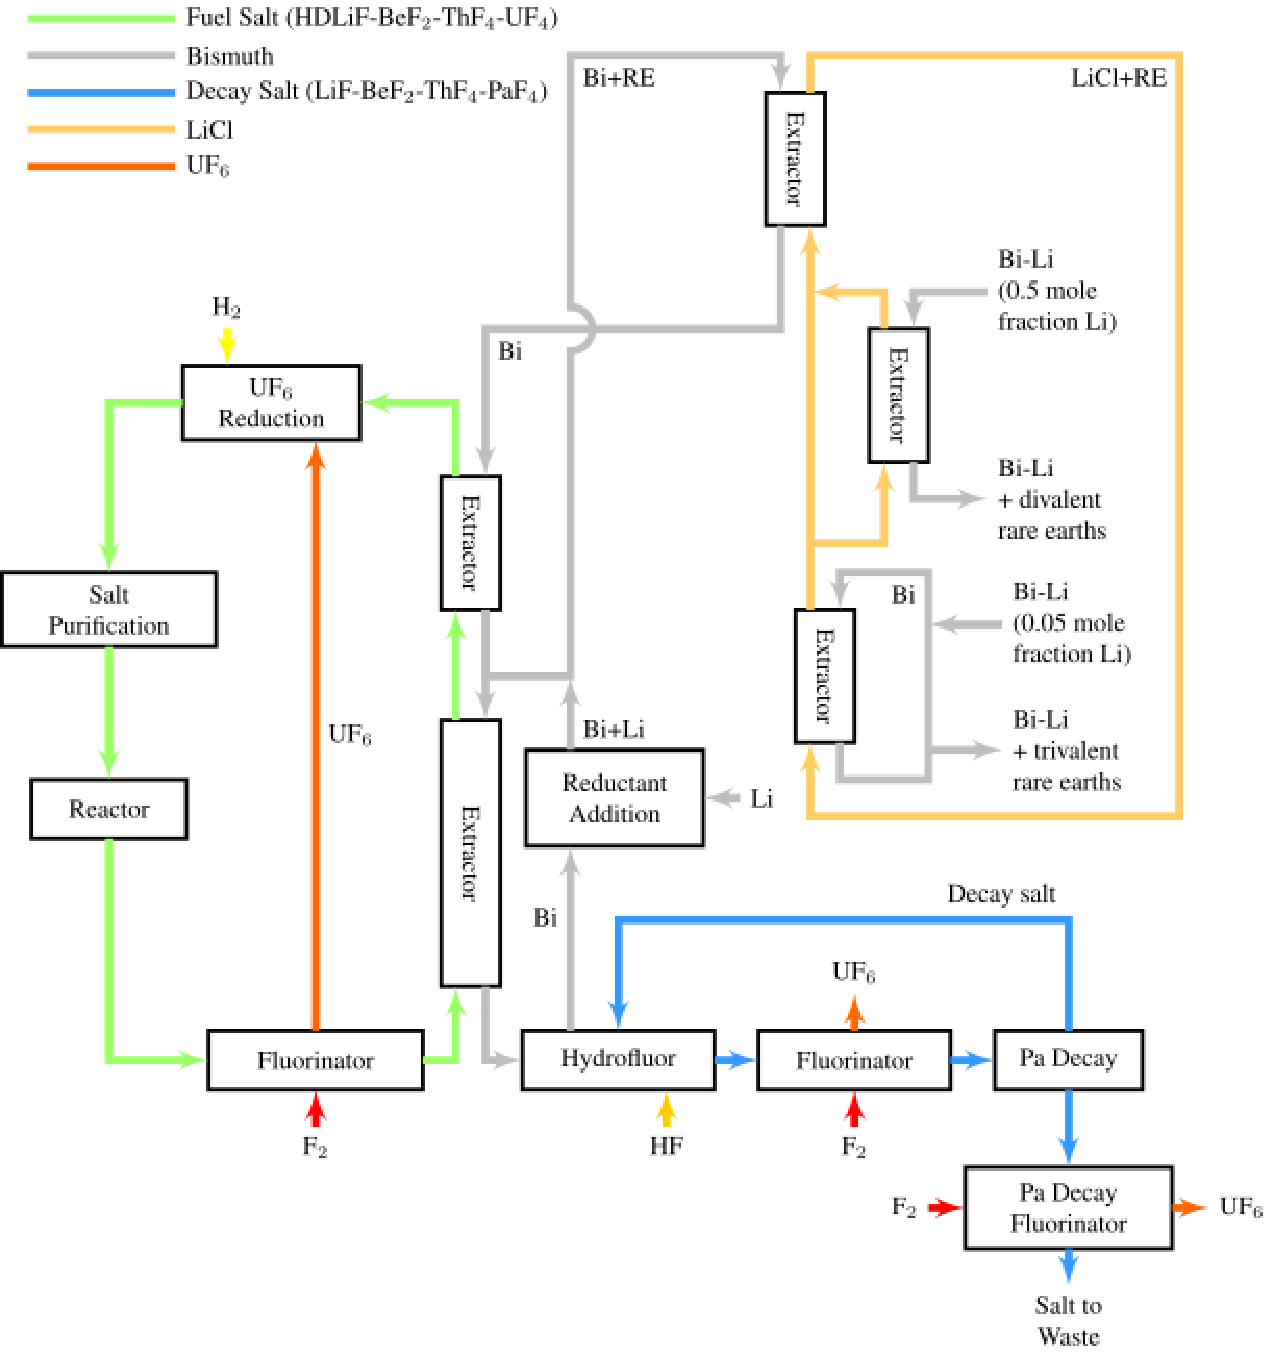
\includegraphics[width=0.57\textwidth]{../figures/flowsheet.pdf}
			\vspace{-2mm}
		\caption{Liquid metal (Bi) extraction system for the \gls{MSBR} 
		(reproduced from Sorensen \cite{sorensen_one-fluid_2006}).} 
	\end{figure}
	
\end{frame}


\begin{frame}
\frametitle{Fuel processing system overview: TAP concept}
	\vspace{-2mm}
\begin{figure}[htp!] % replace 't' with 'b' to 
	\centering
	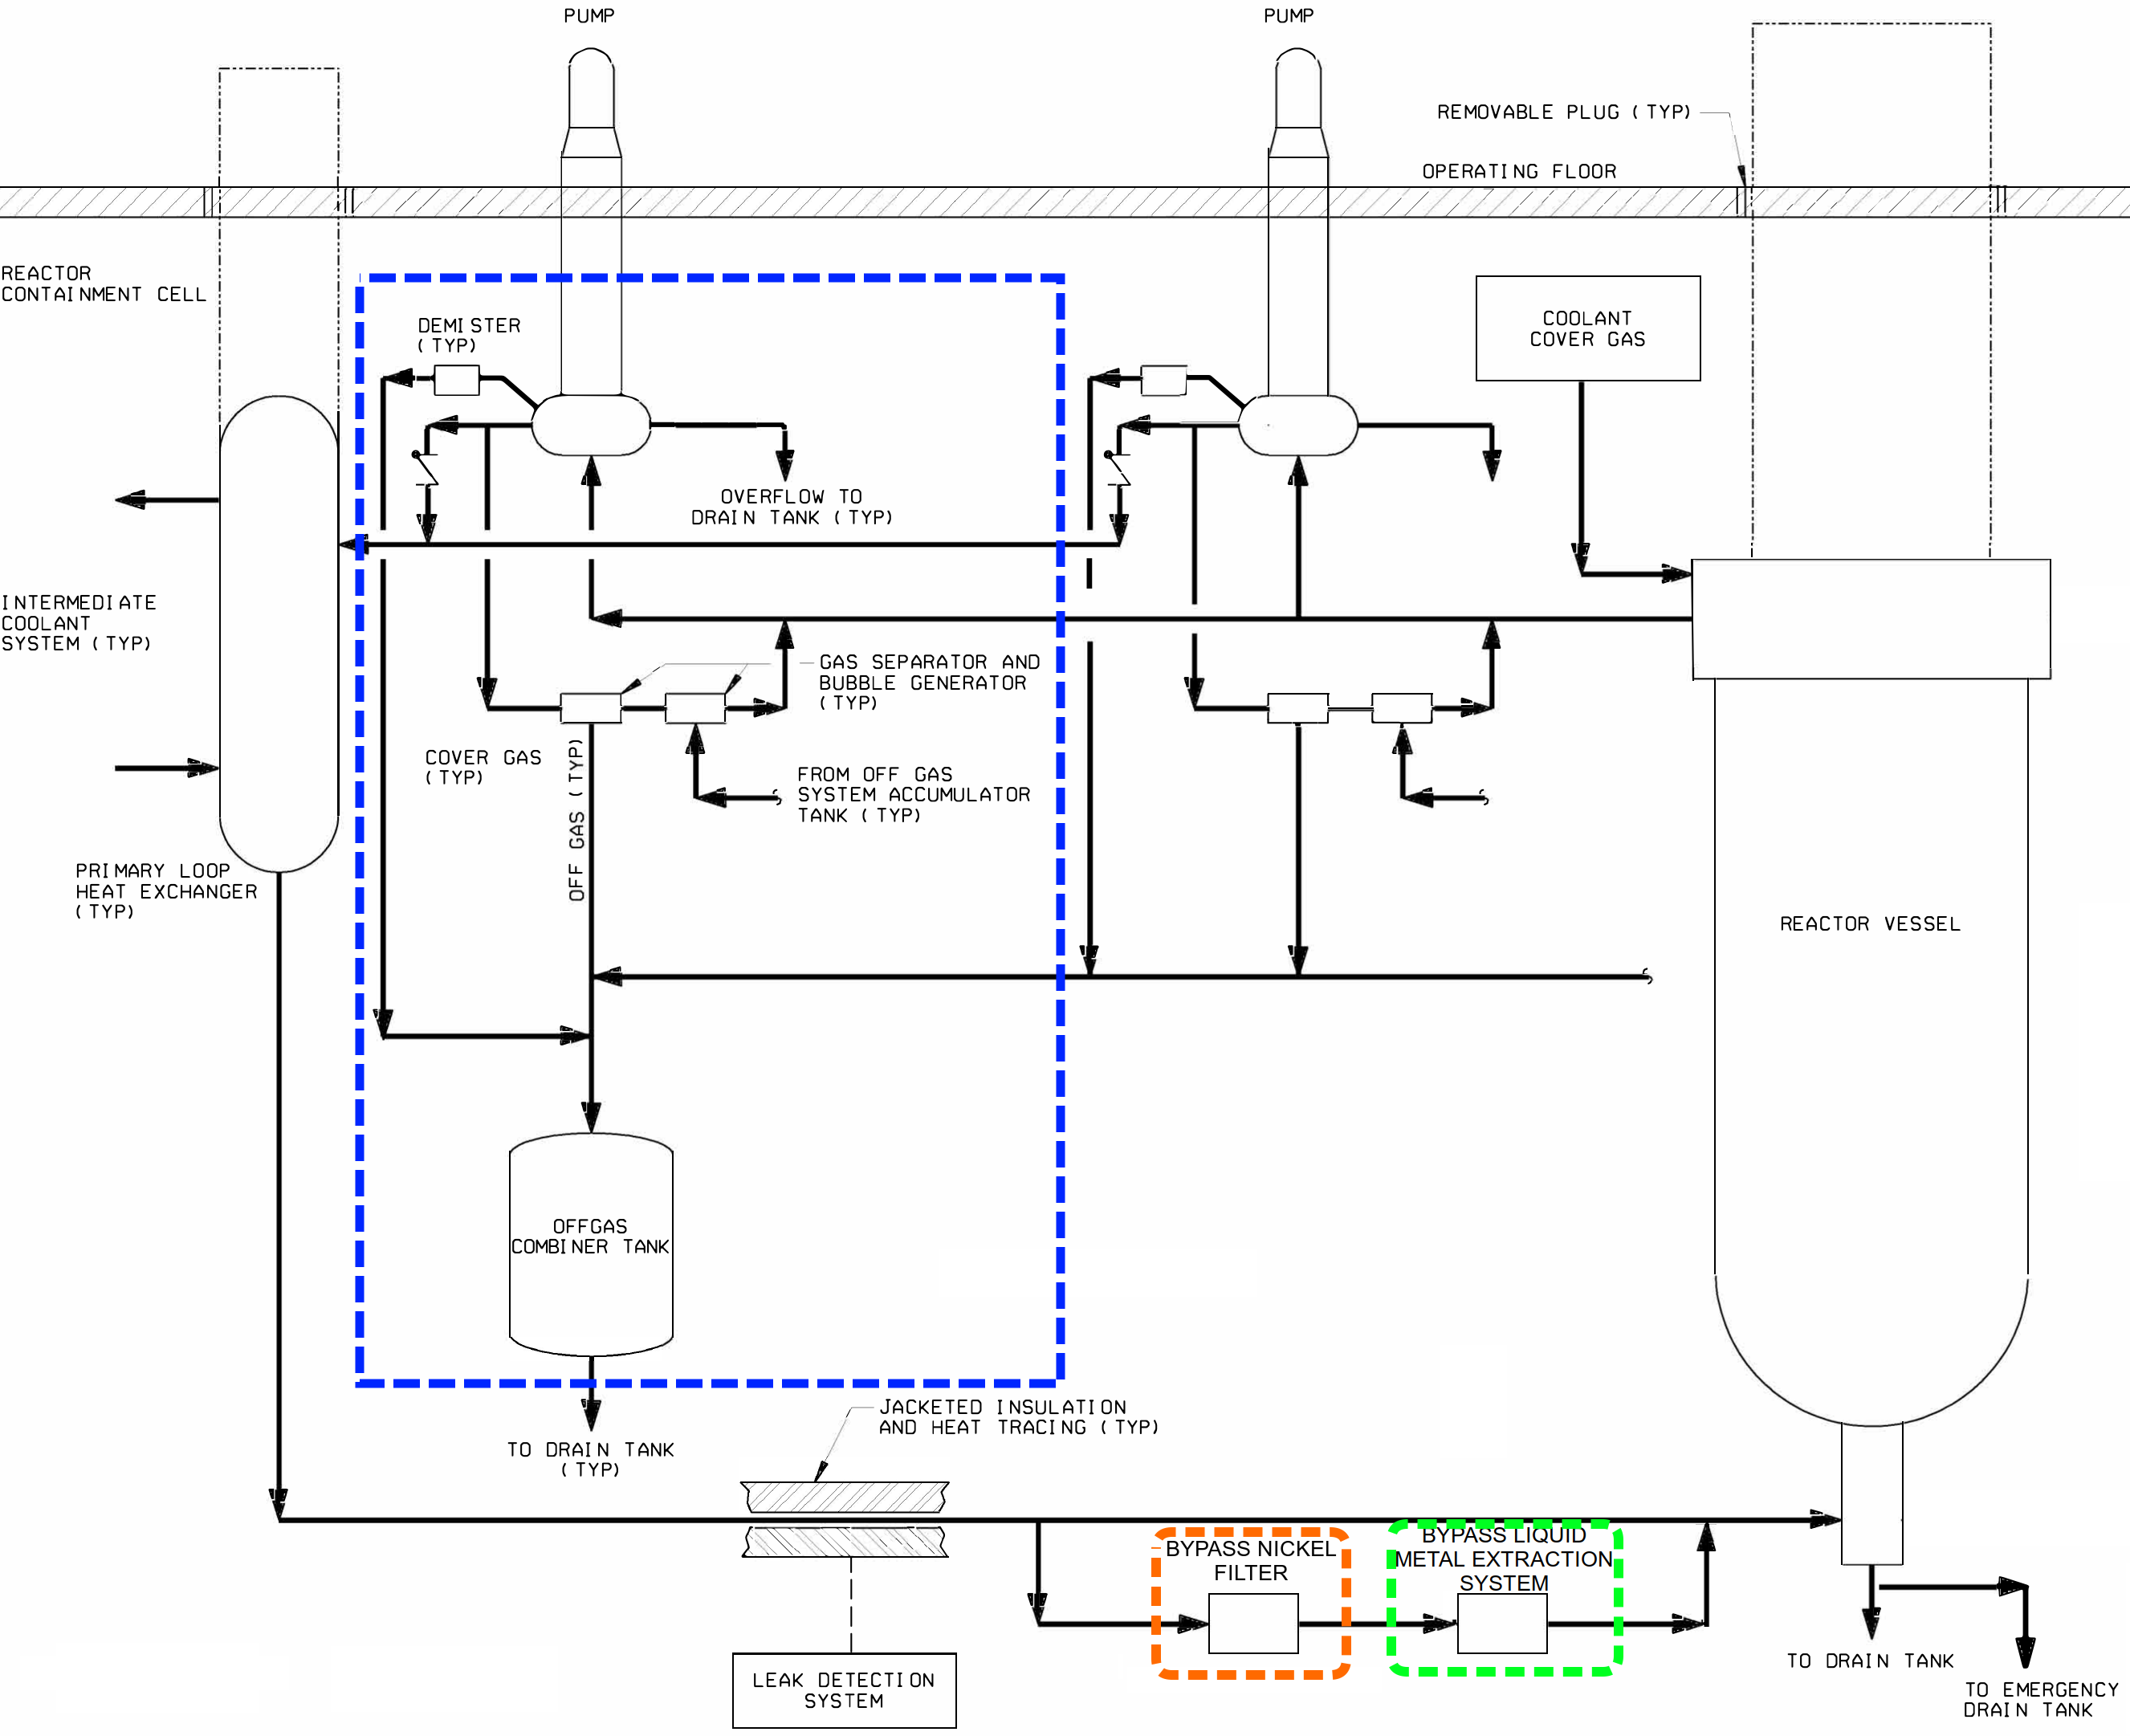
\includegraphics[width=0.75\textwidth]{../figures/tap_primary_loop.png}
	\caption{Simplified \gls{TAP} primary loop design including off-gas system 
		(blue), nickel filter (orange) and liquid metal extraction system 
		(green) \cite{transatomic_power_transatomic_2019}.}
\end{figure}

\end{frame}


\begin{frame}
\frametitle{SaltProc demonstration for TAP concept input data}
	  \begin{textblock*}{12.5cm}(0.5cm,1.5cm) % {block width} (coords)
%%%%%%%%%%%%%%%%%%%%%%%%%%%%%%%%%%%%%%%%
\begin{table}[htbp!]
	\fontsize{6}{9}\selectfont
	\centering
	\caption{The effective cycle times for fission products removal  from the 
		\gls{TAP} reactor \cite{betzler_implementation_2017}.}
	\begin{tabular}{p{0.14\textwidth} p{0.3\textwidth} p{0.11\textwidth} 
			p{0.11\textwidth}}
		\hline 
		\textbf{Processing group} & \qquad\qquad\qquad \textbf{Nuclides} & 
		\textbf{Removal Rate (s$^{-1}$)} & \textbf{Cycle time (at full power)} 
		\\ \hline 
		\multicolumn{3}{c}{\textit{Elements removed in \gls{MSBR} concept and 
				adopted for the \gls{TAP}} \cite{robertson_conceptual_1971}} \\
		Noble gases & Xe, Kr								  & 5.00E-2 & 20 
		sec \\
		Noble metals & Se, Nb, Mo, Tc, Ru, Rh, Pd, Ag, Sb, Te & 5.00E-2 & 20 
		sec \\
		Seminoble metals & Zr, Cd, In, Sn	  				  & 5.79E-8 & 200 
		days\\
		Volatile fluorides & Br, I 							  & 1.93E-7 & 60 
		days\\
		Rare earths & Y, La, Ce, Pr, Nd, Pm, Sm, Gd           & 2.31E-7 & 50 
		days\\
		\qquad & Eu & 2.32E-8 & 500 days \\
		Discard & Rb, Sr, Cs, Ba & 3.37E-9 & 3435 days \\
		\hline
		\multicolumn{3}{c}{\textit{Additional elements removed} 
			\cite{betzler_implementation_2017, 
			transatomic_power_corporation_neutronics_2016}} \\
		Noble gases & H								  	& 5.00E-2 & 20 
		sec    \\
		Noble metals & Ti, V, Cr, Cu						& 3.37E-9 & 3435 
		days \\
		Seminoble metals & Mn, Fe, Co, Ni, Zn, Ga, Ge, As   & 3.37E-9 & 3435 
		days \\
		Rare earths & Sc									& 3.37E-9 & 3435 
		days \\
		Discard & Ca										& 3.37E-9 & 3435 
		days \\
		\hline
	\end{tabular}
	\label{tab:reprocessing_list}
\end{table}
	\begin{itemize}
		\item Noble gas removal efficiency: variable, described using 
		mathematical 
		correlation
		\item Other FPs removal efficiency: fixed, non-ideal, based on 
		Table~\ref{tab:reprocessing_list}
	\end{itemize}
	\end{textblock*}
\end{frame}


\subsection{Proposed tool design}


\begin{frame}
\frametitle{SaltProc architecture}
\vspace{-2mm}
\begin{figure}[ht!] % replace 't' with 'b' to \centering
	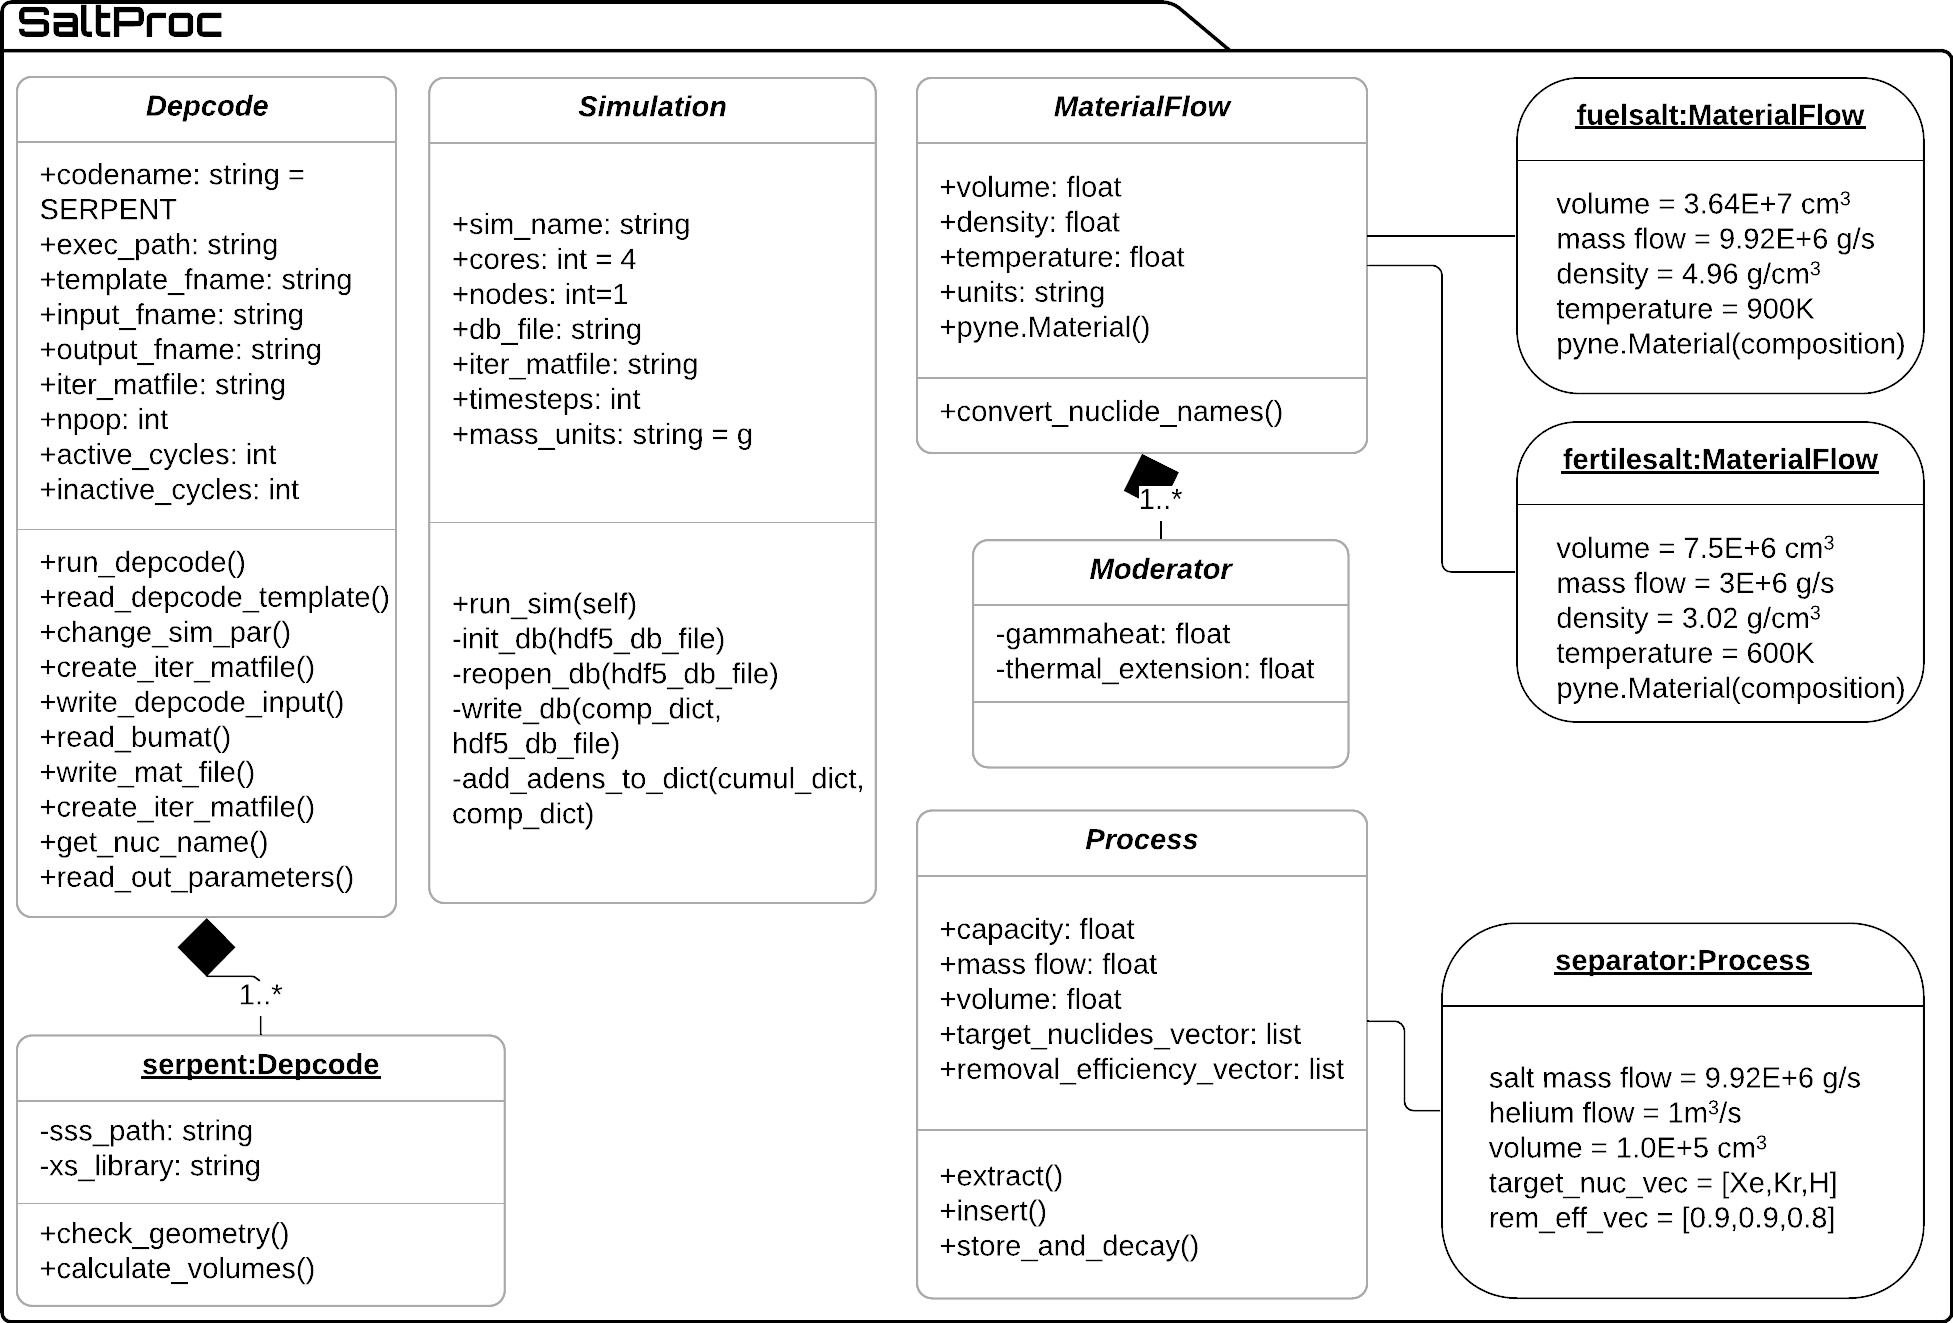
\includegraphics[width=0.84\textwidth]{../figures/saltproc_class_diagram.png}
	\caption{SaltProc v1.0 python package class diagram in UML notation 
		with examples of object instances.}
\end{figure}

\end{frame}


\begin{frame}
\frametitle{SaltProc flowchart}
\vspace{-2mm}
\begin{figure}[ht!] % replace 't' with 'b' to \centering
	\centering
	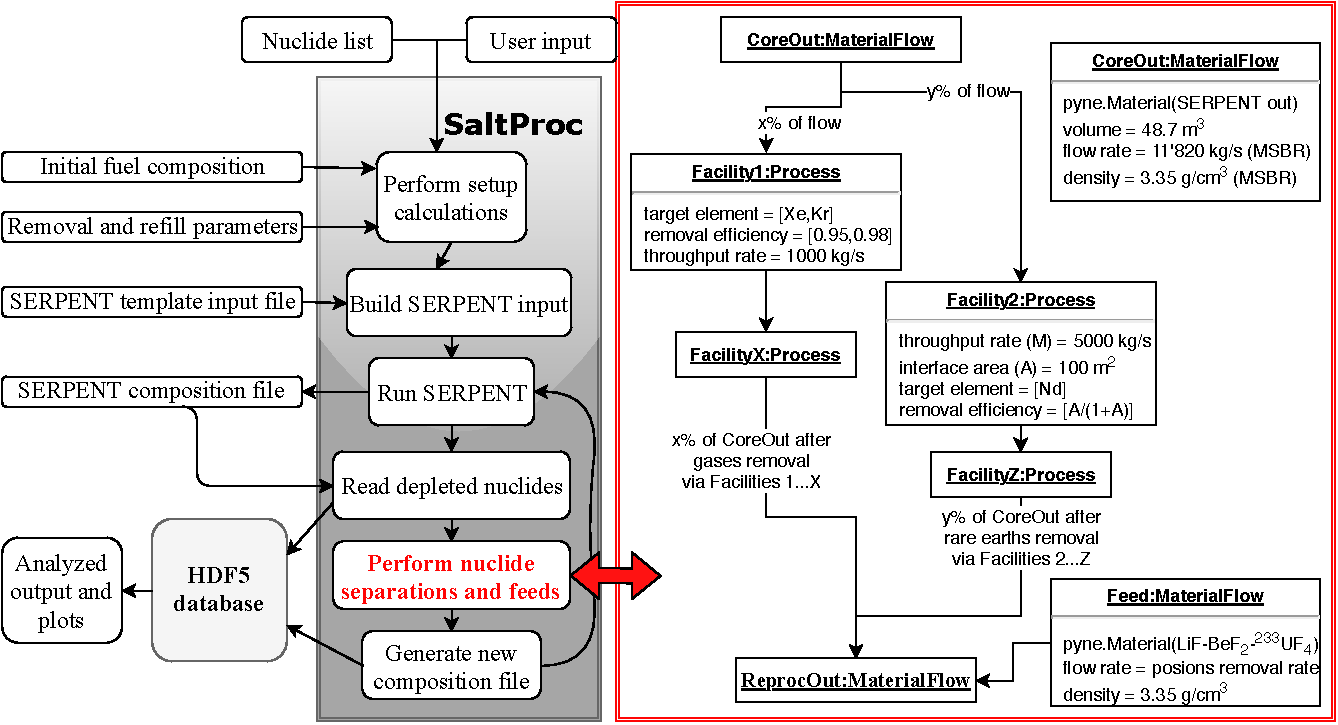
\includegraphics[width=0.95\textwidth]{../figures/saltproc_flowchart.pdf}
	\caption{Tentative generic flowchart for SaltProc v1.0 python package.}
\end{figure}

\end{frame}